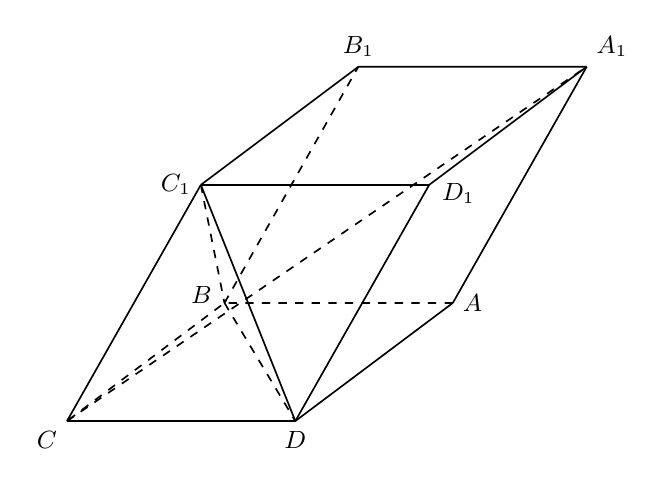
\begin{tikzpicture}[line width=0.6pt, font=\small]
  \coordinate (C) at (0,0);
  \coordinate (D) at (2.9,0);
  \coordinate (A) at (4.9,1.5);
  \coordinate (B) at (2.0,1.5);
  \coordinate (C1) at (1.7,3.0);
  \coordinate (D1) at (4.6,3.0);
  \coordinate (A1) at (6.6,4.5);
  \coordinate (B1) at (3.7,4.5);
  % bottom face: front solid, back dashed
  \draw (C) -- (D) -- (A);
  \draw[dashed] (A) -- (B) -- (C);
  \draw[dashed] (B) -- (D);
  % verticals: front solid, back dashed
  \draw (C) -- (C1);
  \draw (D) -- (D1);
  \draw (A) -- (A1);
  \draw[dashed] (B) -- (B1);
  % top face
  \draw (C1) -- (D1);
  \draw (C1) -- (B1) -- (A1);
  \draw (A1) -- (D1);
  % face diagonal C1D solid, interior diagonals dashed
  \draw (C1) -- (D);
  \draw[dashed] (C1) -- (B);
  
  \draw[dashed] (C) -- (A1);
  % labels
  \node[below left] at (C) {$C$};
  \node[below] at (D) {$D$};
  \node[right] at (A) {$A$};
  \node[left,xshift=-1pt,yshift=3pt] at (B) {$B$};
  \node[left] at (C1) {$C_{1}$};
  \node[right,xshift=1pt,yshift=-3pt] at (D1) {$D_{1}$};
  \node[above right] at (A1) {$A_{1}$};
  \node[above] at (B1) {$B_{1}$};
\end{tikzpicture}
